% Manual de la aplicación web de PULSO, para usuarios sin experiencia previa.
% Compilar desde docs/latex/manual_app:
%   latexmk -lualatex manual_app.tex
\documentclass[11pt,a4paper,oneside]{article}

\usepackage{fontspec}
\usepackage[spanish,es-noshorthands,es-tabla,es-nodecimaldot]{babel}
\usepackage{amsmath,amssymb}
\setmainfont{TeX Gyre Pagella}
\setsansfont{TeX Gyre Heros}
\setmonofont{DejaVu Sans Mono}[Scale=0.82]
\usepackage[margin=2.3cm,headheight=14pt]{geometry}
\usepackage{graphicx}
\usepackage{booktabs,longtable,array}
\usepackage{xcolor}
\usepackage[most]{tcolorbox}
\usepackage{enumitem}
\usepackage{titlesec}
\usepackage{fancyhdr}
\usepackage{caption}
\usepackage{needspace}
\usepackage[hidelinks]{hyperref}

\graphicspath{{../figuras/manual/}{../figuras/}}

\definecolor{azul}{HTML}{2563A8}
\definecolor{rojo}{HTML}{C2362B}
\definecolor{verde}{HTML}{2F7D5B}
\definecolor{ambar}{HTML}{E0A100}
\definecolor{gris}{HTML}{5F6B77}

\titleformat{\section}{\sffamily\bfseries\Large\color{azul}}{\thesection}{0.7em}{}
\titleformat{\subsection}{\sffamily\bfseries\large}{\thesubsection}{0.7em}{}
\titleformat{\subsubsection}{\sffamily\bfseries\normalsize}{}{0em}{}

\pagestyle{fancy}
\fancyhf{}
\fancyhead[L]{\small\sffamily\color{gris}PULSO · manual de la aplicación}
\fancyhead[R]{\small\sffamily\color{gris}\nouppercase{\leftmark}}
\fancyfoot[C]{\small\thepage}
\renewcommand{\headrulewidth}{0.3pt}

\setlength{\parskip}{0.5em}
\setlength{\parindent}{0pt}
\setlist{itemsep=0.15em,topsep=0.25em}
\setlist[description]{font=\normalfont\bfseries,leftmargin=1.2em,labelindent=0em}
\captionsetup{font=small,labelfont=bf}

\newtcolorbox{pruebe}{colback=verde!6,colframe=verde,boxrule=0.5pt,arc=2pt,
  left=6pt,right=6pt,title={\sffamily\small Pruebe esto},fonttitle=\color{black},
  colbacktitle=verde!15,breakable,before upper={\setlength{\parskip}{0.4em}}}
\newtcolorbox{representa}{colback=azul!6,colframe=azul,boxrule=0.5pt,arc=2pt,
  left=6pt,right=6pt,title={\sffamily\small Qué representa},fonttitle=\color{black},
  colbacktitle=azul!15,breakable,before upper={\setlength{\parskip}{0.4em}}}
\newtcolorbox{aviso}{colback=ambar!8,colframe=ambar!80!black,boxrule=0.5pt,arc=2pt,
  left=6pt,right=6pt,title={\sffamily\small Tenga en cuenta},fonttitle=\color{black},
  colbacktitle=ambar!20,breakable,before upper={\setlength{\parskip}{0.4em}}}

% Tabla de controles: control, rango y valor inicial, qué representa
\newenvironment{controles}{%
  \small\setlength{\LTpre}{0.3em}\setlength{\LTpost}{0.3em}
  \begin{longtable}{p{0.2\textwidth}p{0.17\textwidth}p{0.55\textwidth}}
  \toprule
  \textbf{Control} & \textbf{Rango (inicial)} & \textbf{Qué representa y qué pasa al
  cambiarlo} \\
  \midrule
  \endhead}{\bottomrule\end{longtable}}

\newcommand{\captura}[2][0.92]{%
  \begin{center}\fcolorbox{gris!40}{white}{\includegraphics[width=#1\textwidth]{#2}}\end{center}}
\newcommand{\boton}[1]{\fcolorbox{azul}{azul!10}{\sffamily\small #1}}

\hypersetup{pdftitle={PULSO: manual de la aplicación},pdfauthor={Juan Diego Martínez Ayala}}

\begin{document}

\begin{titlepage}
\centering
\vspace*{2.5cm}
{\sffamily\bfseries\Huge\color{azul} PULSO\par}
\vspace{0.2cm}
{\sffamily\large\color{gris} Pagos, Umbrales, Liquidez y Sincronización Operativa\par}
\vspace{0.9cm}
{\sffamily\LARGE Manual de la aplicación\par}
\vspace{0.4cm}
{\large Guía página por página para quien la usa por primera vez:\\
qué hace cada control y qué representa cada resultado\par}
\vspace{1.2cm}
\fcolorbox{gris!40}{white}{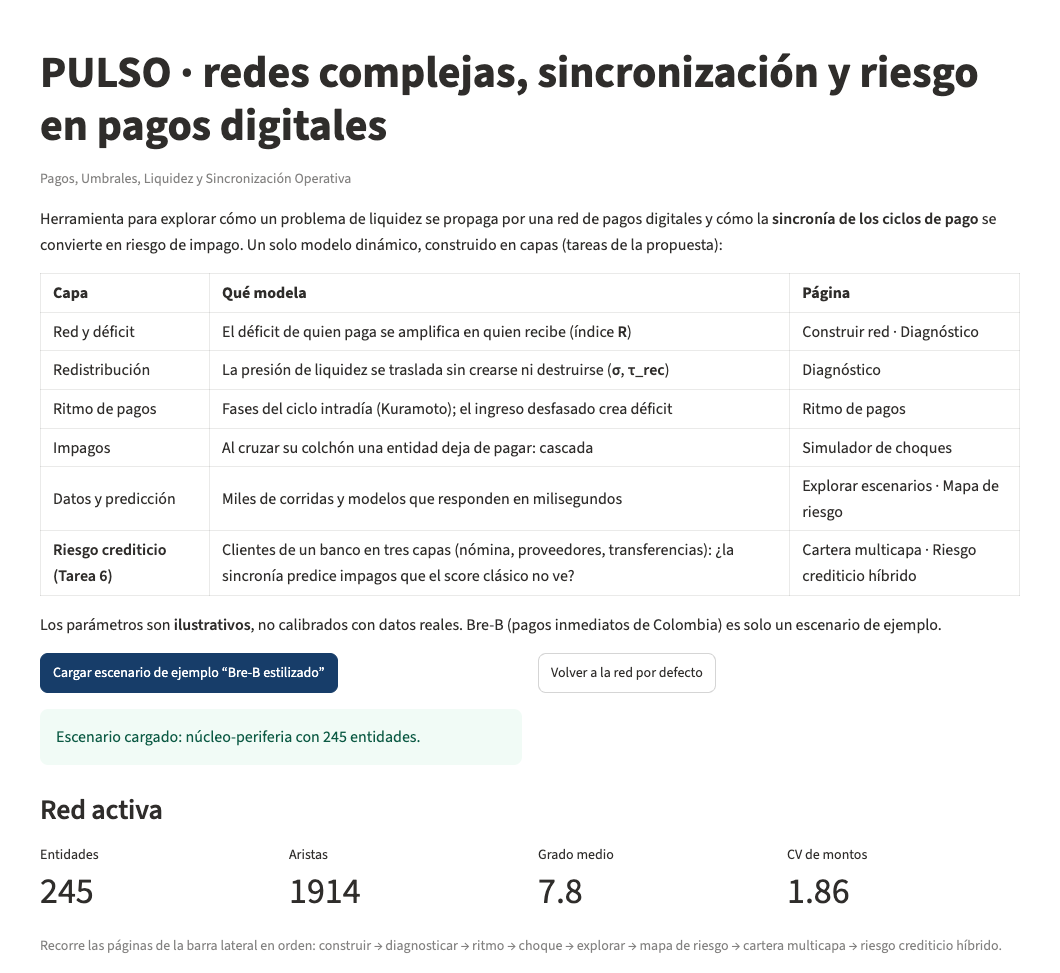
\includegraphics[width=0.7\textwidth]{inicio_1.png}}\par
\vfill
{\large Juan Diego Martínez Ayala\par}
{\normalsize Semillero de Modelamiento de Sistemas Complejos y Física Computacional\par}
\vspace{0.4cm}
{\normalsize Noviembre de 2026 · software v3.1.0\par}
\end{titlepage}

\tableofcontents
\clearpage

% ===================================================================
\section{Qué es la aplicación}

La aplicación de PULSO es un laboratorio interactivo. Permite construir una red de
pagos, aplicarle un choque y ver cómo se propaga, sin escribir código. También muestra
los resultados del proyecto sobre riesgo de crédito.

Tiene diez páginas en dos bloques:

\begin{center}
\small
\begin{tabular}{p{0.32\textwidth}p{0.6\textwidth}}
\toprule
\textbf{Páginas} & \textbf{Para qué sirven} \\
\midrule
Inicio & Presentación y carga del escenario de ejemplo. \\
1 Construir red & Crear la red de pagos con la que trabajan las páginas 2 a 7. \\
2 Diagnóstico & Saber si la red amortigua o amplifica un choque. \\
3 Ritmo de pagos & Ver cómo se sincronizan los ciclos de pago. \\
4 Simulador de choques & Aplicar un choque y ver la cascada de impagos. \\
5 Explorar escenarios & Consultar 20\,000 simulaciones ya hechas. \\
6 Mapa de riesgo & Predicción instantánea del riesgo de cada entidad. \\
7 Acerca del modelo & Ecuaciones, supuestos y límites. \\
\midrule
8 Cartera multicapa & Clientes de un banco en tres capas de pagos (tarea 6). \\
9 Riesgo crediticio híbrido & Comparar el score clásico con el modelo que usa la red
(tarea 6). \\
\bottomrule
\end{tabular}
\end{center}

Las páginas 1 a 7 trabajan con una \textbf{red de entidades}: bancos, empresas o
participantes de un sistema de pagos, sin distinguir su tipo. Las páginas 8 y 9 trabajan
con una \textbf{cartera de clientes} de un banco: personas y empresas.

\begin{aviso}
Todos los datos son simulados y los parámetros son ilustrativos. La aplicación sirve
para entender mecanismos, no para medir el riesgo de una institución real.
\end{aviso}

% ===================================================================
\section{Cómo abrir la aplicación}

\subsection{En el computador, con uv}
En una terminal, dentro de la carpeta del proyecto:
\begin{verbatim}
uv sync                              # solo la primera vez: instala todo
uv run streamlit run app/Inicio.py   # abre la aplicación
\end{verbatim}
El navegador se abre en \texttt{http://localhost:8501}. Si ese puerto está ocupado,
use otro puerto y abra \texttt{http://localhost:8502}:
\begin{verbatim}
uv run streamlit run app/Inicio.py --server.port=8502
\end{verbatim}

\subsection{Con Docker}
\begin{verbatim}
docker build -t pulso .
docker run -p 8501:8501 pulso
\end{verbatim}
y abra \texttt{http://localhost:8501}. La imagen ya trae los datos y los modelos
entrenados.

\subsection{Para cerrarla}
Cierre la pestaña del navegador y, en la terminal, presione \texttt{Ctrl+C}.

% ===================================================================
\section{Elementos de la pantalla}

\begin{description}
\item[Barra lateral.] A la izquierda. Tiene la lista de páginas y, debajo, un resumen de
la red activa (topología, número de entidades y aristas) o de la cartera activa
(personas, firmas, informalidad y semilla). Se oculta con la flecha \texttt{<<}.
\item[Deslizador.] Barra con un punto que se arrastra para elegir un número. El valor
actual aparece encima. Con el teclado, las flechas lo mueven paso a paso.
\item[Formulario.] Recuadro con varios controles y un botón azul (\boton{Construir},
\boton{Simular}, \boton{Simular cartera}). Los cambios dentro del recuadro no tienen
efecto hasta presionar el botón. Así se pueden cambiar varios valores a la vez sin
esperar una simulación por cada uno.
\item[Control fuera de formulario.] Se aplica al soltarlo: la página se recalcula de
inmediato.
\item[Métrica.] Número grande con su nombre encima. Algunas tienen un símbolo
\textbf{?}: al pasar el cursor muestra una explicación. Debajo puede aparecer una
flecha con la diferencia respecto a un caso de referencia.
\item[Gráfica interactiva.] Al pasar el cursor sobre un punto se ve su información. Con
el ratón se puede hacer zoom arrastrando un rectángulo; doble clic restablece la vista.
En la esquina superior derecha hay botones para descargar la imagen, mover, ampliar y
ver en pantalla completa. Al hacer clic en un elemento de la leyenda se oculta o se
muestra esa serie.
\item[Tabla.] Al hacer clic en el nombre de una columna se ordena por ella.
\item[Desplegable (\emph{expander}).] Línea con una flecha \texttt{>} que se abre al
hacer clic y muestra contenido adicional.
\item[Indicador de ejecución.] Mientras la aplicación calcula, en la esquina superior
derecha aparece un aviso de ejecución. Espere a que desaparezca antes de leer los
resultados.
\end{description}

\subsection{Estado compartido entre páginas}
La red que se construye en \emph{Construir red} y los parámetros que se ajustan en
\emph{Diagnóstico}, \emph{Ritmo de pagos} y \emph{Simulador de choques} se comparten.
Por ejemplo, el valor de $\alpha$ elegido en \emph{Diagnóstico} se usa también en el
simulador. Lo mismo ocurre con la cartera de la página 8, que usa la página 9.

El estado dura mientras la pestaña esté abierta. Si se recarga la página del navegador,
todo vuelve a los valores iniciales.

\subsection{Límite de tamaño}
Con más de 300 entidades, las páginas que simulan en vivo (\emph{Diagnóstico}, en su
choque de prueba; \emph{Ritmo de pagos}; \emph{Simulador de choques}; y la verificación
del \emph{Mapa de riesgo}) se desactivan y muestran un aviso. La barra lateral también lo
indica. El \emph{Mapa de riesgo} sigue funcionando porque predice sin simular.

% ===================================================================
\section{Conceptos mínimos}

Estos términos aparecen en todas las páginas.

\begin{description}
\item[Entidad o nodo.] Un participante de la red. Se dibuja como un círculo.
\item[Arista.] Una flecha de pago de una entidad a otra. Su peso es el pago medio por
ciclo.
\item[Ciclo.] Unidad de tiempo de las páginas 1 a 7: un ciclo de pagos, equivalente a un
día hábil. En las páginas 8 y 9 la unidad es el mes.
\item[Pago medio.] Unidad de dinero de las páginas 1 a 7. Los montos están escalados para
que la arista promedio valga 1.
\item[Déficit ($x$).] Faltante de liquidez de una entidad. Cero significa sin problemas.
\item[Colchón (umbral).] Déficit máximo que una entidad soporta. Si lo supera, entra en
impago.
\item[Impago.] La entidad deja de pagar a todos sus receptores.
\item[Cascada.] Impagos en cadena: el impago de una entidad lleva a otras a superar su
colchón.
\item[Fase ($\theta$).] Momento del ciclo de pagos en que está una entidad, como la
posición de la manecilla de un reloj.
\item[Sincronía ($r$).] Qué tan alineados están los ciclos. $r=1$: todos pagan al mismo
tiempo. $r=0$: cada uno a su ritmo.
\item[Semilla.] Número que fija el azar. Con la misma semilla se obtiene exactamente el
mismo resultado.
\item[PD.] Probabilidad de impago de un cliente en los próximos doce meses.
\end{description}

% ===================================================================
\section{Inicio}

\captura{inicio_1.png}

La página de inicio resume el modelo en una tabla. Cada fila es una capa del modelo,
lo que modela y la página donde se explora.

\begin{description}
\item[\boton{Cargar escenario de ejemplo “Bre-B estilizado”}.] Reemplaza la red y los
parámetros por un escenario de ejemplo: red núcleo-periferia de 245 entidades (del orden
de los participantes de Bre-B en su primer año), grado medio 8, índice de amplificación
$R=0.85$, redistribución $D_0=0.05$, acople $K=3$ y colchón $0.5$. Los valores son
ilustrativos.
\item[\boton{Volver a la red por defecto}.] Restaura la red inicial: núcleo-periferia de
80 entidades, grado medio 6, $R=0.8$, semilla 42.
\end{description}

Debajo, cuatro métricas describen la red activa:

\begin{description}
\item[Entidades.] Número de nodos.
\item[Aristas.] Número de relaciones de pago dirigidas.
\item[Grado medio.] Número medio de pagadores (o de receptores) por entidad.
\item[CV de montos.] Coeficiente de variación de los montos: desviación estándar
dividida por la media. Un valor alto indica pocos pagos muy grandes y muchos pequeños.
\end{description}

% ===================================================================
\section{Construir red}

\captura{construir_1.png}

\begin{representa}
Un sistema de pagos como red. Cada círculo es una entidad y cada línea un pago
recurrente. El tamaño del círculo es proporcional al volumen de pagos. En la topología
núcleo-periferia, los círculos rojos son el núcleo: las grandes entidades que concentran
los pagos.
\end{representa}

\subsection*{Controles (dentro del formulario)}
\begin{controles}
Topología & Erdős–Rényi, Barabási–Albert, Núcleo-periferia (núcleo-periferia) &
Forma de la red. \textbf{Erdős–Rényi}: conexiones al azar, todas las entidades parecidas.
\textbf{Barabási–Albert}: unas pocas entidades muy conectadas (concentradores).
\textbf{Núcleo-periferia}: un núcleo denso y una periferia conectada a él; es la forma de
los sistemas de pagos reales. \\
Número de entidades & 10 a 600 (80) & Tamaño de la red. Por encima de 300 se desactiva la
simulación en vivo. \\
Grado medio & 1 a 20 (6) & Número medio de contrapartes de cada entidad. Más grado, red
más densa. Debe ser menor que el número de entidades menos uno. \\
Dispersión de montos ($\sigma$ lognormal) & 0 a 2 (0.8) & Desigualdad de los montos. Con
0 todos los pagos valen igual; con valores altos aparecen pagos muy grandes. \\
Fracción en el núcleo & 0.02 a 0.40 (0.10) & Proporción de entidades del núcleo. Solo se
activa con núcleo-periferia. \\
Semilla & 0 a $10^6$ (42) & Fija el azar de la construcción. Cambiarla produce otra red
con las mismas características. \\
\end{controles}

Al presionar \boton{Construir} se genera la red. Las simulaciones previas se borran
porque correspondían a la red anterior.

\subsection*{Resultados}
\begin{description}
\item[Entidades y aristas dirigidas.] Tamaño de la red.
\item[Densidad.] Fracción de las conexiones posibles que existen, entre 0 y 1.
\item[CV de montos.] Ver \emph{Inicio}.
\item[Gráfica de la red.] Al pasar el cursor sobre una entidad se ve cuánto paga y
cuánto recibe por ciclo.
\end{description}

\begin{pruebe}
Construya una red Barabási–Albert de 100 entidades y luego una Erdős–Rényi del mismo
tamaño y grado. En la primera verá unos pocos círculos grandes en el centro; en la
segunda, círculos de tamaño parecido. Después vaya a \emph{Diagnóstico}: con el mismo
$\beta$, la red Barabási–Albert tendrá un $R$ mayor.
\end{pruebe}

% ===================================================================
\section{Diagnóstico}

\captura{diagnostico_1.png}

\begin{representa}
La salud de la red frente a un choque, calculada sin simular, a partir de los valores
propios de la red. Responde: si una entidad sufre un déficit, ¿la red lo absorbe o lo
amplifica? ¿Cuánto tarda en recuperarse? ¿Qué entidades son más importantes?
\end{representa}

\subsection*{Controles}
\begin{controles}
$\alpha$ · autocorrección [1/ciclo] & 0.05 a 3 (1.0) & Rapidez con que cada entidad
corrige su déficit por sí misma. $1/\alpha$ es el tiempo típico de corrección. Subirlo
estabiliza la red. \\
$\beta$ · amplificación & 0 a $2\alpha/\rho$ (el que da $R=0.8$) & Déficit que genera en
una entidad el déficit de quien le paga. El rango se ajusta a la red para que $R$ vaya de
0 a 2. Subirlo desestabiliza la red. \\
$D_0$ · redistribución & 0 a 2 (0) & Traslado de presión de liquidez de una entidad a sus
receptores sin crearla ni destruirla. Acelera la recuperación. \\
Comunidades & 2 a 8 (3) & Número de grupos en que se divide la red para colorearla. \\
\end{controles}

\subsection*{Resultados}
\begin{description}
\item[Índice de amplificación $R$.] $R=\beta\rho(W)/\alpha$, donde $\rho(W)$ es el radio
espectral de la red (su valor propio dominante). $R<1$: la red amortigua. $R>1$: la red
amplifica. Es el análogo del número reproductivo de una epidemia.
\item[Estabilidad $\sigma$ con semáforo.] Mayor parte real de los valores propios de
$M=-\alpha I-D_0L+\beta W$. Incluye la redistribución, así que es más completo que $R$.
\textcolor{verde}{Verde}: $\sigma<-0.05$, la red amortigua.
\textcolor{ambar}{Amarillo}: $|\sigma|\le0.05$, la red está cerca del límite y los
choques tardan mucho en disiparse. \textcolor{rojo}{Rojo}: $\sigma>0.05$, el déficit
crece sin límite.
\item[Tiempo de recuperación.] $\tau_\text{rec}=-1/\sigma$, en ciclos: tiempo en que un
choque se reduce a un 37~\% ($1/e$). Aparece $\infty$ si la red no se recupera.
\item[Conectividad algebraica $\lambda_2$.] Mide qué tan bien conectada está la red como
un todo. Vale 0 si está partida en pedazos aislados. Mayor $\lambda_2$, más rápida la
redistribución.
\item[Comunidades.] Gráfica con la red coloreada por grupos que se pagan mucho entre sí y
poco con el resto. Se obtienen con el vector de Fiedler (bisección espectral).
\item[Ranking por vector propio dominante.] Las 15 entidades más importantes.
\emph{importancia}: cuánto déficit propaga si entra en problemas (vector propio
izquierdo). \emph{vulnerabilidad}: cuánto déficit acumula si otros entran en problemas
(vector propio derecho). \emph{paga} y \emph{recibe}: flujos por ciclo.
\end{description}

\captura{diagnostico_2.png}

\subsection*{Choque de prueba (sin impagos)}
Aplica un retiro de liquidez a una entidad y muestra cómo evoluciona el déficit, sin
umbrales: nadie entra en impago. Sirve para ver la estabilidad en acción.

\begin{controles}
Entidad chocada & 0 a $n-1$ (la más importante) & Entidad que sufre el choque. \\
Tamaño & 0.1 a 10 ciclos (2) & Déficit inicial, medido en ciclos de los pagos salientes
de la entidad: 2 equivale a dos ciclos de lo que paga. \\
\end{controles}

\begin{description}
\item[Trayectorias.] El déficit de cada entidad en el tiempo; la entidad chocada aparece
resaltada.
\item[Déficit total del sistema ($\Sigma x$).] Suma de todos los déficits. Con $R<1$
termina en cero; con $R>1$ crece.
\end{description}

\begin{pruebe}
Mueva $\beta$ hasta que $R$ pase de 0.9 a 1.1. El semáforo cambia de verde a rojo y el
déficit total del choque de prueba deja de bajar y empieza a crecer. Luego suba $D_0$:
$\sigma$ baja y la red puede volver a ser estable aunque $R>1$.
\end{pruebe}

% ===================================================================
\section{Ritmo de pagos}

\captura{ritmo_1.png}

\begin{representa}
Cada entidad paga en ciclos, como un reloj que da vueltas. La posición en la vuelta es
su fase. Cada entidad tiene su propio ritmo, pero tiende a ajustarlo al de quienes le
pagan. La página muestra si las entidades terminan sincronizadas y cuánto déficit se
genera cuando el ingreso llega desfasado.
\end{representa}

\subsection*{Controles}
\begin{controles}
$K$ · dependencia de fondos entrantes & 0 a 10 (2) & Intensidad con que cada entidad
ajusta su ritmo al de quienes le pagan. Más $K$, más sincronía. \\
$\Delta$ · dispersión de ritmos naturales & 0 a 2 (0.5) & Qué tan distintos son los
ritmos propios de las entidades. Más $\Delta$, más difícil sincronizar. \\
$\gamma$ · peso de la desincronización en el déficit & 0 a 0.5 (0) & Cuánto déficit genera
el ingreso desfasado. Con 0, la sincronía no afecta la liquidez. \\
Desconectar entidad a mitad de la corrida & ninguna o una de las 30 que más pagan &
Elimina todos los pagos de esa entidad en la mitad de la simulación (ciclo 10 de 20). \\
\end{controles}

\subsection*{Resultados}
\begin{description}
\item[$r$ final.] Parámetro de orden al final: 0 si las fases están dispersas, 1 si todas
coinciden. Con una desconexión, la flecha muestra la diferencia frente a la red
completa.
\item[Déficit total final.] Suma de los déficits al final. Con desconexión, muestra la
diferencia.
\item[Coherencia local media.] Promedio de $r_i$, que mide si a cada entidad le llega el
ingreso en fase (1), sin relación (0) o en contrafase ($-1$).
\item[Círculo de fases.] Animación: cada punto es una entidad sobre un círculo según su
fase. Si se agrupan, están sincronizadas. Use el botón de reproducción.
\item[Parámetro de orden $r(t)$.] Evolución de la sincronía. Con desconexión se muestran
dos curvas: con y sin la entidad.
\item[Déficit total.] Evolución de la suma de déficits.
\item[Coherencia local al final.] Red coloreada por $r_i$: verde, ingreso en fase; rojo,
en contrafase.
\end{description}

\captura[0.8]{ritmo_2.png}

\begin{aviso}
Con $\gamma=0$ aparece un mensaje: las fases se sincronizan, pero el déficit no cambia.
Suba $\gamma$ para ver el efecto del ritmo sobre la liquidez.
\end{aviso}

\begin{pruebe}
Con $\gamma=0.1$, mueva $K$ de 0 a 6. Con $K$ bajo, $r$ queda cerca de 0 y el déficit
total crece; con $K$ alto, $r$ se acerca a 1 y el déficit se reduce. Después desconecte la
primera entidad de la lista: $r$ cae y el déficit sube en la segunda mitad.
\end{pruebe}

% ===================================================================
\section{Simulador de choques}

\captura{simulador_1.png}

\begin{representa}
Un choque sobre una entidad y la cascada de impagos que provoca. A diferencia del
choque de prueba de \emph{Diagnóstico}, aquí sí hay colchones: la entidad que los supera
deja de pagar y sus receptores pierden ingreso. Usa los parámetros $\alpha$, $\beta$,
$D_0$, $K$ y $\gamma$ elegidos en las páginas anteriores.
\end{representa}

\subsection*{Controles (dentro del formulario)}
\begin{controles}
Entidad chocada & todas, ordenadas por lo que pagan & Entidad que recibe el choque. Junto
al número aparece cuánto paga por ciclo. \\
Tipo de choque & Retiro de liquidez o Caída operativa & \textbf{Retiro de liquidez}: un
salto súbito en el déficit, como una retirada masiva de depósitos. \textbf{Caída
operativa}: la entidad sigue recibiendo pero no paga durante un tiempo, como una falla
tecnológica. \\
Tamaño del retiro & 0.1 a 10 ciclos (2) & Solo para el retiro: déficit inicial en ciclos
de pagos salientes. \\
Duración de la caída $T$ & 0.5 a 15 ciclos (3) & Solo para la caída operativa: cuánto
dura sin pagar. \\
Colchón $c$ & 0.05 a 3 (0.5) & Reserva de cada entidad, medida en ciclos de sus pagos
salientes. Más colchón, menos impagos. \\
$\lambda$ · pérdida por ingreso no recibido & 0 a 3 (1) & Cuánto déficit genera perder un
pagador. Con 1, perder todo el ingreso equivale a un ciclo de los pagos propios. \\
\end{controles}

El choque ocurre en el ciclo 1 y la simulación dura 20 ciclos.

\subsection*{Resultados}
\begin{description}
\item[En impago.] Porcentaje de entidades que terminan en impago. El símbolo \textbf{?}
muestra el número.
\item[Liquidez no pagada.] Pagos que no se hicieron por los impagos, acumulados, en pagos
medios.
\item[DebtRank.] Medida clásica del daño sistémico (Battiston et al., 2012), entre 0 y
1: fracción del valor económico de la red afectada por el estrés, sin contar a la
entidad chocada.
\item[Primer contagio.] Ciclo en que cae la primera entidad distinta de la chocada.
``—'' si no hubo contagio.
\item[Colapso global.] Mensaje rojo si cae el 30~\% o más de la red.
\item[Animación de la cascada.] Red coloreada por estado: \textcolor{verde}{verde}, sin
problemas; \textcolor{ambar}{ámbar}, en estrés (déficit mayor que la mitad de su
colchón); \textcolor{rojo}{rojo}, en impago. La entidad chocada tiene borde negro. Use el
botón de reproducción o arrastre la barra de tiempo.
\item[Línea de tiempo de eventos.] Cada punto es un impago: en el eje horizontal el
ciclo y en el vertical la entidad.
\item[Liquidez no pagada acumulada.] Evolución en el tiempo del indicador anterior.
\item[\boton{Exportar indicadores y eventos (CSV)}.] Descarga los resultados en un
archivo que se abre con Excel.
\end{description}

\begin{aviso}
Si $\gamma>0$ algunas entidades pueden caer antes del choque por la desincronización.
Un mensaje lo indica; esas caídas no cuentan como contagio.
\end{aviso}

\captura{simulador_2.png}

\subsection*{Entidades más peligrosas}
El botón \boton{Calcular ranking} choca, una por una, cada entidad con el tamaño elegido
y mide la fracción media de las demás que caen (\emph{cascada\_media}). Muestra las 10 más
peligrosas. Tarda unos segundos y el resultado queda guardado mientras no cambie la
configuración.

\begin{pruebe}
Choque la entidad que más paga con un retiro de 3 ciclos y colchón 0.5. Anote el
porcentaje en impago. Suba el colchón a 1.0 y repita: la cascada se reduce mucho.
Luego compare un retiro con una caída operativa de 3 ciclos sobre la misma entidad.
\end{pruebe}

% ===================================================================
\section{Explorar escenarios}

\captura{explorar_1.png}

\begin{representa}
Los resultados de 20\,000 simulaciones hechas de antemano sobre 300 redes distintas,
con parámetros variados. Permite responder preguntas generales sin simular: ¿en qué
condiciones colapsa una red? ¿Qué topología es más frágil?
\end{representa}

\begin{aviso}
Requiere el conjunto de datos. Si no existe, la página indica el comando para generarlo:
\texttt{uv run pulso sweep configs/sweep.yaml} (unos 20 minutos).
\end{aviso}

\subsection*{Filtros (en el desplegable \emph{Filtros})}
\begin{controles}
Topología & las tres (todas) & Redes que se incluyen. \\
Tipo de choque & liquidez, operativo (ambos) & Choques que se incluyen. \\
Índice de amplificación $R$ & 0.4 a 1.6 (todo) & Rango de $R$. \\
Grado medio & 2 a 12 (todo) & Rango de conectividad. \\
Colchón $c$ & 0.2 a 1.5 (todo) & Rango de colchones. \\
Acople $K$ & 0 a 6 (todo) & Rango de acople de fase. \\
\end{controles}

\subsection*{Resultados}
\begin{description}
\item[Corridas filtradas.] Número de simulaciones que cumplen los filtros.
\item[P(colapso).] Porcentaje de ellas con colapso global (30~\% o más en impago).
\item[Fracción media en impago.] Promedio del porcentaje de entidades que caen.
\item[Liquidez no pagada media.] En ciclos de flujo total del sistema.
\item[Ventana de contagio.] Fracción en impago contra grado medio, por topología. Muestra
que las cascadas son mayores con conectividad intermedia: con pocas conexiones el choque
no se propaga; con muchas, cada entidad diversifica su ingreso y absorbe la pérdida.
\item[Fracción en impago contra $R$.] Cada punto es una simulación (máximo 3000). Por
encima de $R=1$ aparecen las cascadas grandes.
\item[Distribución del tamaño de cascada.] Histograma por tipo de choque. La mayoría de
los choques se absorben; unos pocos producen colapsos.
\end{description}

\captura{explorar_2.png}

\subsection*{Comparar escenarios lado a lado}
Elija hasta cuatro escenarios por su número (por defecto, los dos con mayor cascada). La
tabla muestra sus parámetros y resultados en columnas. \boton{Exportar filtro (CSV)}
descarga todos los escenarios filtrados.

\begin{pruebe}
Filtre $R$ entre 0.4 y 0.9 y observe P(colapso). Luego filtre $R$ entre 1.1 y 1.6. La
probabilidad de colapso aumenta mucho. Compare también las tres topologías por separado.
\end{pruebe}

% ===================================================================
\section{Mapa de riesgo}

\captura{mapa_1.png}

\begin{representa}
El riesgo de cada entidad de la red activa, predicho por modelos de aprendizaje
automático entrenados con las 20\,000 simulaciones. La predicción tarda milisegundos;
simular cada entidad tardaría minutos. El riesgo de una entidad es el daño que causaría si
sufriera un retiro de 3 ciclos.
\end{representa}

\begin{aviso}
Requiere los modelos entrenados. Si no existen, la página indica el comando:
\texttt{uv run pulso train configs/train.yaml}.
\end{aviso}

\subsection*{Controles}
\begin{controles}
Modelo & Cascada (GCN), Cascada (XGBoost), P(colapso global) & Qué riesgo colorea la red.
\textbf{Cascada}: fracción de las demás entidades que caerían. La \textbf{GCN} es una red
neuronal que lee la estructura del grafo; \textbf{XGBoost} es un conjunto de árboles de
decisión. \textbf{P(colapso global)}: probabilidad de que caiga el 30~\% o más de la red.
\\
Entidad (sección SHAP) & todas, de mayor a menor riesgo & Entidad cuya predicción se
explica. \\
\end{controles}

\subsection*{Resultados}
\begin{description}
\item[Riesgo predicho por entidad.] Red coloreada de amarillo (bajo) a rojo (alto).
\item[Tabla.] Las 12 entidades más riesgosas con las tres predicciones y lo que pagan.
\item[Contribuciones SHAP.] Barras que explican la predicción de XGBoost para la entidad
elegida. Parten de un valor base (el riesgo promedio) y cada barra suma o resta riesgo:
\textcolor{rojo}{rojo} aumenta, \textcolor{azul}{azul} reduce. Los nombres de las variables
se explican en la tabla siguiente.
\item[\boton{Verificar con simulación}.] Simula de verdad el choque sobre la entidad y
compara el resultado (\emph{Simulado}) con las predicciones de la GCN y de XGBoost. La
flecha muestra el error de cada modelo.
\item[Métricas de validación.] Desplegable con el desempeño de los modelos fuera de
muestra.
\end{description}

\subsection*{Variables del gráfico SHAP}
\begin{center}
\small
\begin{longtable}{p{0.24\textwidth}p{0.68\textwidth}}
\toprule
\textbf{Variable} & \textbf{Significado} \\
\midrule
\endhead
\texttt{in\_degree}, \texttt{out\_degree} & Número de pagadores y de receptores. \\
\texttt{in\_amount}, \texttt{out\_amount} & Ingreso y pagos por ciclo. \\
\texttt{importance}, \texttt{vulnerability} & Importancia y vulnerabilidad espectrales
(ver \emph{Diagnóstico}). \\
\texttt{pagerank} & Centralidad PageRank. \\
\texttt{r\_local} & Coherencia local de fase antes del choque. \\
\texttt{threshold} & Colchón de la entidad. \\
\texttt{out\_share} & Fracción de todos los pagos del sistema que hace la entidad. \\
\texttt{shock\_to\_buffer} & Tamaño del choque dividido por el colchón propio. Mayor que 1:
la entidad cae con el choque. \\
\texttt{max\_dependency} & Mayor fracción del ingreso que algún receptor obtiene de esta
entidad. \\
\texttt{downstream\_impact} & Suma, sobre los receptores, de la pérdida que sufrirían
dividida por su colchón. \\
\texttt{first\_order\_defaults} & Fracción de entidades que caerían solo por la primera
ronda de pérdidas. \\
\texttt{debtrank} & DebtRank de un choque en la entidad. \\
\texttt{n}, \texttt{topology}, \texttt{R}, \texttt{sigma}, \texttt{K}, \texttt{gamma},
\texttt{buffer}, \texttt{loss} & Características de toda la red y del modelo: tamaño,
topología, amplificación, estabilidad, acople, desfase, colchón y pérdida. \\
\bottomrule
\end{longtable}
\end{center}

\begin{aviso}
Las predicciones solo son confiables dentro de los rangos con que se entrenaron los
modelos (los del archivo \texttt{configs/sweep.yaml}). El orden de las entidades dentro de
una misma red es aproximado; para una decisión, use \boton{Verificar con simulación}.
\end{aviso}

\begin{pruebe}
Elija la entidad más riesgosa, lea sus barras SHAP y presione \boton{Verificar con
simulación}. Compare el valor simulado con las dos predicciones.
\end{pruebe}

% ===================================================================
\section{Acerca del modelo}

\captura{acerca_1.png}

Página de consulta, sin controles. Contiene:

\begin{itemize}
\item Las ecuaciones del modelo de las páginas 1 a 7: déficit, ritmo de pagos e impago.
\item Una tabla con el significado de cada símbolo.
\item La unidad de tiempo, el integrador y la definición de los dos tipos de choque.
\item Los supuestos y límites: parámetros ilustrativos, redes sintéticas, acople en un
solo sentido, modelo lineal hasta el umbral y validez de las predicciones solo dentro de
los rangos de entrenamiento.
\item Las ecuaciones de la tarea 6 (páginas 8 y 9), el control nulo y las referencias.
\end{itemize}

% ===================================================================
\section{Cartera multicapa}

\captura{cartera_1.png}

\begin{representa}
Los clientes de un banco: personas (círculos) y empresas (cuadrados). Están unidos por
tres tipos de pago: \textbf{nómina} (empresa a empleado), \textbf{proveedores} (empresa a
empresa) y \textbf{transferencias} (persona a persona). Cada cliente tiene un ciclo de
pagos. Si su ingreso le llega desfasado de su propio ciclo, acumula déficit.

El banco no ve los ciclos: solo ve las transacciones. La página muestra el modelo
interno y lo que se estima a partir de las transacciones. El tiempo se mide en meses.
\end{representa}

\subsection*{Controles (dentro del formulario)}
\begin{controles}
Personas & 100 a 600 (400) & Número de personas de la cartera. \\
Firmas & 5 a 40 (20) & Número de empresas. \\
Informalidad & 0 a 0.9 (0.55) & Fracción de personas sin empleador en el banco. Los
informales tienen ritmos de pago más irregulares. \\
Semilla & 0 a 10\,000 (7) & Fija el azar: misma semilla, misma cartera. \\
Mundo & con red / nulo & \textbf{Con red}: la red transmite déficit (contagio, desfase y
pérdida de ingreso). \textbf{Nulo}: control; los pagos existen pero la red no crea
déficit. Mismos clientes y mismo azar. \\
$K$ nómina & 0 a 3 (0.8) & Cuánto ajusta un empleado su ritmo de pagos al de su
empleador. \\
$\gamma$ & 0 a 2 (0.5) & Cuánto déficit genera el ingreso desfasado. Con 0, la sincronía
no afecta el riesgo. \\
\end{controles}

\subsection*{Resultados principales}
\begin{description}
\item[Clientes.] Personas más empresas.
\item[$R=\rho(B)/\alpha$.] Índice de amplificación de la cartera. Menor que 1: la red
amortigua. En el mundo nulo vale 0.
\item[Impago en observación.] Porcentaje de clientes que caen en los primeros 6 meses
(ventana de observación).
\item[Impago a 12 meses.] Entre los que siguen activos a los 6 meses, porcentaje que cae en
los 12 meses siguientes. Es la etiqueta que predicen los modelos.
\item[Sincronía final $\hat r$.] Sincronía global de toda la cartera estimada desde las
transacciones. Suele ser baja porque las empresas pagan en fechas distintas: lo que
importa para el riesgo es la coherencia de cada cliente con sus propios pagadores, no la
de toda la cartera.
\item[Gráfica de la cartera.] El selector \emph{Color} cambia lo que se pinta:
\emph{coherencia local $\hat r$} (verde, ingreso en fase; rojo, desfasado),
\emph{impago a 12 meses} (rojo, cayó) o \emph{tipo de cliente}. Las líneas tienen el color
de su capa.
\item[Capas.] Tabla con el número de relaciones y el monto mensual de cada capa, en
salarios mínimos (SMMLV) por mes.
\item[Sincronía global de la cartera.] Curva gris: sincronía real del modelo, que el
banco no ve. Curva roja: la estimada desde las transacciones. La línea punteada marca el
fin de la observación (mes 6); la curva roja solo existe antes.
\end{description}

\captura{cartera_2.png}

\subsection*{¿Quién está desincronizado?}
\begin{description}
\item[Coherencia local $\hat r$ por grupo.] Diagramas de caja para empresas, personas
formales e informales, solo con clientes que reciben ingreso por la red. La caja abarca la
mitad central de los clientes y la línea es la mediana. Los formales están cerca de 1
(sincronizados con su nómina); los informales, cerca de 0.
\item[Impago a 12 meses según $\hat r$.] Tasa de impago por tramos de coherencia, con los
resultados del experimento completo de 20 carteras. En rojo el mundo con red; en gris el
nulo. El número sobre cada barra es la cantidad de clientes.
\end{description}

\begin{aviso}
En el mundo nulo también hay más impago con $\hat r$ bajo, porque los informales son más
riesgosos y están menos sincronizados. Por eso esta gráfica no prueba la hipótesis. La
prueba está en la comparación de modelos de la página siguiente.
\end{aviso}

\subsection*{Escenario: quiebra de un empleador}
\begin{controles}
Firma que quiebra en $t=1$ mes & las 8 con más empleados & Empresa que deja de pagar todo
(nómina, proveedores y cuota) en el primer mes. Se muestra su número de empleados en el
banco. \\
\end{controles}
Al presionar \boton{Simular quiebra} aparecen:
\begin{description}
\item[Empleados que caen (6 meses).] Porcentaje de sus empleados en impago entre el mes 1
y el 7, con la diferencia frente a la misma cartera sin quiebra.
\item[Resto de personas.] Mismo porcentaje para las demás personas.
\item[Empleados afectados.] Número de empleados de la firma.
\item[Clientes en impago acumulados.] Curvas con y sin quiebra.
\end{description}
En el mundo nulo la quiebra no transmite déficit y un mensaje lo recuerda.

\subsection*{Registro de transacciones}
El desplegable muestra las primeras 500 transacciones: lo que el banco ve. Columnas:
\texttt{t} (mes), \texttt{src} (pagador), \texttt{dst} (receptor; $-1$ es el banco, es
decir, una cuota), \texttt{layer} y \texttt{capa} (tipo de pago), \texttt{amount} (monto en
SMMLV). El botón descarga todas en CSV.

\begin{pruebe}
Con la cartera por defecto, simule la quiebra de la firma más grande en el mundo con red
y anote el porcentaje de empleados que caen. Cambie a mundo nulo y repita: la diferencia
desaparece. Después ponga $\gamma=0$ en el mundo con red y observe el color por $\hat r$:
la sincronía sigue igual, pero deja de afectar el impago.
\end{pruebe}

% ===================================================================
\section{Riesgo crediticio híbrido}

\captura{hibrido_1.png}

\begin{representa}
La respuesta a la pregunta del proyecto: ¿la sincronía de los ciclos de pago predice
impagos que el score clásico y la red estática no ven? Compara tres niveles de
variables con el mismo modelo y las mismas particiones:
\begin{enumerate}
\item \textbf{Clásico}: ingreso, endeudamiento, moras, antigüedad, empleo formal.
\item \textbf{+ Red estática}: de quién y cuánto recibe, concentración del ingreso,
PageRank, salud del empleador y de los pagadores.
\item \textbf{+ Red dinámica}: coherencia con los pagadores, desfase, ritmo,
irregularidad de los ciclos, pagadores que dejaron de pagar.
\end{enumerate}
\end{representa}

\begin{aviso}
Requiere los resultados del experimento. Si no existen, ejecute
\texttt{uv run pulso credit configs/credit.yaml} (menos de un minuto).
\end{aviso}

\subsection*{Control}
\begin{controles}
Modelo & XGBoost o Regresión logística & Modelo con que se comparan los niveles en la
parte superior. La regresión logística es el modelo clásico de los bancos; XGBoost
combina árboles de decisión. \\
\end{controles}

\subsection*{Comparación de niveles}
\begin{description}
\item[Dinámica vs.\ red estática ($\Delta$AUC).] Cuánto mejora el AUC al agregar las
variables dinámicas a las estáticas, en el mundo con red. Debajo, el intervalo de
confianza del 95~\%: si no incluye el cero, la mejora es significativa.
\item[Híbrido vs.\ clásico ($\Delta$AUC).] Mejora total del modelo con todas las variables
sobre el score clásico.
\item[Control nulo.] La misma comparación en el mundo nulo. Debe ser cercana a cero. Si
no lo fuera, habría una fuga de información.
\item[AUC fuera de muestra.] Barras por mundo y nivel. El AUC es la probabilidad de que el
modelo asigne más riesgo a un cliente que cae que a uno que no cae: 0.5 es azar, 1 es
perfecto. Las líneas negras son la variación entre particiones.
\item[PR-AUC.] Métrica similar, más exigente cuando los impagos son pocos. Un modelo al
azar obtiene la tasa de impago (cerca de 0.1).
\item[Mejoras pareadas por partición.] Cada fila es una comparación con su intervalo de
confianza. En verde, las que están por encima de cero.
\item[Tabla completa de métricas.] Desplegable con AUC, PR-AUC, KS (separación entre
buenos y malos pagadores), Brier y ECE (calibración: menor es mejor).
\end{description}

\captura{hibrido_2.png}

\subsection*{Riesgo por cliente en la cartera activa}
Usa la cartera de la página \emph{Cartera multicapa} (personas, firmas, informalidad y
semilla), siempre en el mundo con red y con los valores de $K$ y $\gamma$ del archivo de
configuración, no los de los deslizadores. Las probabilidades salen de modelos XGBoost
finales entrenados con las 20 carteras del experimento.

\begin{description}
\item[PD a 12 meses: score clásico vs.\ híbrido.] Cada punto es un cliente activo. Eje
horizontal: probabilidad de impago según el score clásico. Eje vertical: según el modelo
híbrido. \textcolor{rojo}{Rojo}: el cliente cayó; \textcolor{verde}{verde}: no cayó.
Cuadrados: empresas. Los puntos por encima de la diagonal son clientes que el híbrido ve
más riesgosos que el clásico.
\item[Riesgo oculto.] Los 10 clientes cuyo riesgo más sube al mirar la red, con ambas PD y
si cayeron.
\item[Tasa de impago en el 10~\% más riesgoso.] De los clientes que cada modelo marca
como el 10~\% más riesgoso, cuántos cayeron. Con una sola cartera pequeña esta cifra
varía mucho; la comparación válida es la de la parte superior.
\end{description}

\captura{hibrido_3.png}

\subsection*{¿Por qué? Contribuciones SHAP}
\begin{description}
\item[Importancia media $|$SHAP$|$.] Las 15 variables que más pesan en el modelo híbrido.
Gris: clásicas. Azul: red estática. Rojo: red dinámica.
\item[Explicar un cliente.] Elija un cliente (primero aparecen los de riesgo oculto). Las
barras muestran qué sube (rojo) y qué baja (verde) su riesgo, en log-odds: la escala en
que el modelo suma contribuciones.
\item[\boton{Descargar PD por cliente (CSV)}.] Descarga ambas PD de todos los clientes.
\end{description}

\begin{pruebe}
Cambie el modelo entre XGBoost y regresión logística: la conclusión se mantiene. Después
abra el cliente con mayor riesgo oculto y vea qué variables de red explican el aumento.
\end{pruebe}

% ===================================================================
\section{Recorridos guiados}

Tres recorridos cortos que muestran los resultados principales del proyecto.

\subsection{De la estabilidad a la cascada (10 minutos)}
\begin{enumerate}
\item En \emph{Inicio}, presione \boton{Volver a la red por defecto}.
\item En \emph{Diagnóstico}, deje $\alpha=1$ y mueva $\beta$ hasta $R\approx0.8$. El
semáforo está en verde.
\item Vaya a \emph{Simulador de choques}. Choque la entidad que más paga con un retiro de
3 ciclos y colchón 0.5. Anote el porcentaje en impago.
\item Vuelva a \emph{Diagnóstico}, suba $\beta$ hasta $R\approx1.2$ (semáforo rojo) y repita
el choque. La cascada es mucho mayor.
\item Suba el colchón a 1.2 y repita. La cascada se reduce: el colchón es la defensa de
cada entidad.
\end{enumerate}

\subsection{La ventana de contagio (5 minutos)}
\begin{enumerate}
\item En \emph{Explorar escenarios}, deje todos los filtros abiertos.
\item Observe la gráfica \emph{Ventana de contagio}: la fracción en impago es máxima con
grado medio intermedio.
\item Filtre solo choques de liquidez y luego solo operativos, y compare.
\end{enumerate}

\subsection{La sincronía como riesgo (10 minutos)}
\begin{enumerate}
\item En \emph{Cartera multicapa}, simule la cartera por defecto en el mundo con red y
coloree por coherencia $\hat r$. Los formales aparecen verdes; los informales, amarillos o
rojos.
\item Revise los diagramas de caja de \emph{¿Quién está desincronizado?}.
\item Simule la quiebra del mayor empleador y compare con el mundo nulo.
\item En \emph{Riesgo crediticio híbrido}, lea las tres métricas superiores: la dinámica
mejora a la red estática en el mundo con red y no mejora nada en el nulo.
\item Abra el cliente con mayor riesgo oculto y lea sus barras SHAP.
\end{enumerate}

% ===================================================================
\section{Solución de problemas}

\begin{longtable}{p{0.36\textwidth}p{0.58\textwidth}}
\toprule
\textbf{Síntoma} & \textbf{Causa y solución} \\
\midrule
\endhead
\emph{Red demasiado grande para simulación en vivo} & La red tiene más de 300 entidades.
Redúzcala en \emph{Construir red} o use el \emph{Mapa de riesgo}. \\
\emph{El grado medio debe ser menor que n - 1} & El grado pedido es imposible para ese
tamaño. Baje el grado o suba el número de entidades. \\
\emph{No hay dataset} (Explorar escenarios) & Ejecute \texttt{uv run pulso sweep
configs/sweep.yaml}. \\
\emph{No hay modelos entrenados} (Mapa de riesgo) & Ejecute \texttt{uv run pulso train
configs/train.yaml}. \\
\emph{No hay resultados del experimento} (páginas 8 y 9) & Ejecute \texttt{uv run pulso
credit configs/credit.yaml}. \\
La página no cambia al mover un control & Si el control está dentro de un formulario,
presione su botón azul. Espere a que desaparezca el indicador de ejecución. \\
Los valores volvieron a los iniciales & Se recargó la pestaña del navegador. El estado
dura solo mientras la pestaña esté abierta. \\
\emph{Port 8501 is already in use} & Otra aplicación usa el puerto. Agregue
\texttt{--server.port=8502}. \\
\emph{ModuleNotFoundError: No module named 'pulso'} (macOS) & macOS oculta un archivo de
la instalación dentro de \texttt{\textasciitilde/Documents}. Ejecute
\texttt{chflags -R nohidden .venv} o anteponga \texttt{PYTHONPATH=src} al comando. \\
Una simulación tarda mucho & Redes grandes o tiempos largos. La primera vez cada
cálculo tarda más; después queda guardado en memoria. \\
\bottomrule
\end{longtable}

% ===================================================================
\section{Glosario rápido}

\begin{longtable}{p{0.24\textwidth}p{0.7\textwidth}}
\toprule
\textbf{Término} & \textbf{Significado} \\
\midrule
\endhead
$\alpha$ & Velocidad con que una entidad corrige su déficit. \\
$\beta$ & Intensidad del contagio de déficit entre pagador y receptor. \\
$\gamma$ & Déficit que genera el ingreso desfasado. \\
$\Delta$ & Dispersión de los ritmos naturales de pago. \\
$\lambda$ & Déficit que genera perder un pagador. \\
$\lambda_2$ & Conectividad algebraica de la red. \\
$\sigma$ & Estabilidad: negativa, la red se recupera; positiva, amplifica. \\
$\tau_\text{rec}$ & Tiempo de recuperación tras un choque. \\
$D_0$ & Intensidad de la redistribución de liquidez. \\
$K$ & Intensidad con que se ajustan los ritmos de pago. \\
$R$ & Índice de amplificación; menor que 1, la red amortigua. \\
$r$, $\hat r$ & Sincronía real y estimada desde transacciones. \\
AUC & Capacidad de un modelo para ordenar a los que caen por encima de los que no. \\
Colapso global & Impago del 30~\% o más de la red. \\
DebtRank & Medida del daño sistémico de un choque. \\
GCN & Red neuronal que trabaja sobre grafos. \\
Mundo nulo & Control en que la red no transmite déficit. \\
PD & Probabilidad de impago a 12 meses. \\
SHAP & Método que explica cuánto aporta cada variable a una predicción. \\
SMMLV & Salario mínimo mensual legal vigente. \\
XGBoost & Modelo de aprendizaje automático basado en árboles de decisión. \\
\bottomrule
\end{longtable}


\end{document}
